\chapter{Methodology} \label{chap:methodology}

This chapter will present a multi-level model design flow for the integration of heterogeneous applications and their deployment to the edge on embedded low power devices like NVIDIA Jetson TX2.


\section{A ROS based robotic system}
The choice of the most suitable integration platform is one of the main problems to be faced when integrating heterogeneous applications such as robotic software systems. This choice will have implications on performance and communication of the whole system. Furthermore it will be a key factor during the design phase of the entire architecture.
After an accurate comparison among all available robotics platforms, for the purpose of the specific application developed in this thesis it has been decided to use ROS \cite{ROS} in favour of its standard on communication among other robotic applications.


The design flow proposed in this work is composed of three bottom-up architecture levels, but the same methodology can be applied with more levels.
The purpose of this methodology is to bring an heterogeneous application within an orchestration system such as Kubernetes, and then extend it to the edge computing. % embedded systems
The architecture are explained in the next sections.




\section{First level architecture}
This is the first architecture to start with.
At this architecture level the purpose is to verify the functioning of the whole system with the only ROS capabilities on a single powerful machine. A simple scheme of this architecture is shown in figure \ref{fig:l1arch}.

\begin{figure}[htbp]
	\centering
	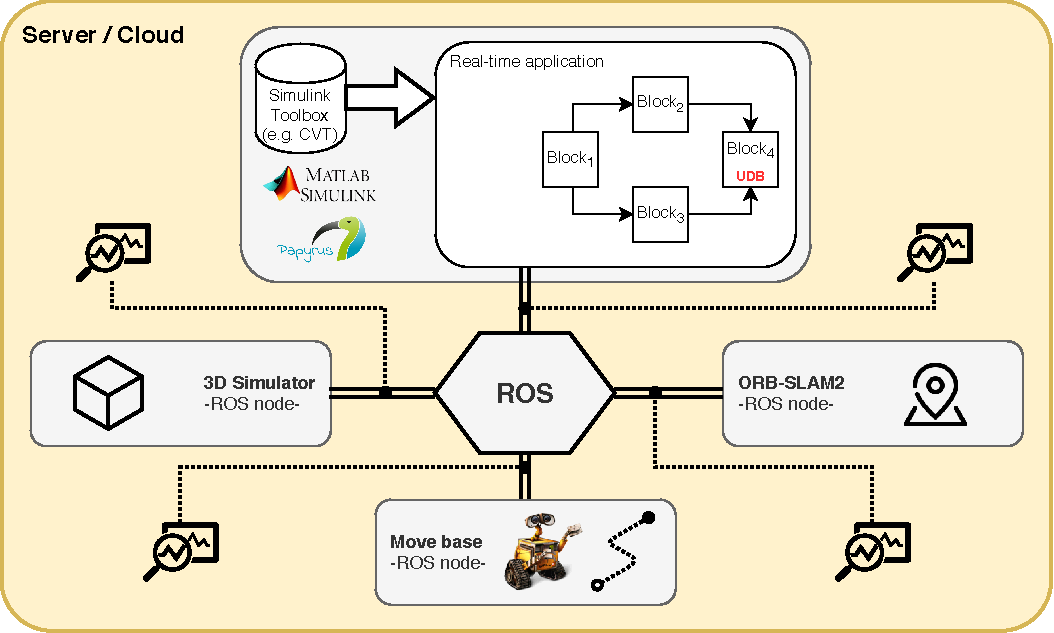
\includegraphics[width=\textwidth]{images/L1-arch}
	\caption{L1 architecture}
	\label{fig:l1arch}
\end{figure}

The first step to realize this architecture is to wrap your (heterogeneous) applications with the ROS conformance protocol advertises and callbacks. An example of this operation is provided in listings \ref{lst:pub} and \ref{lst:sub}.
In this way, all the applications that compose your system will be able to communicate among them following the standard communication based on ROS.
The ROS nodes (publishers and subscribers) communicate between them through topics, thus it is necessary choice the right names of these topics and who will read/write on them.
Once the applications are ready to run on ROS, they can be executed using a launchfile, where the user can specify a set of nodes to launch and their parameters.
Another possibility is invoke the \lstinline{rosrun} command for each node that have to be executed.


\noindent\begin{minipage}{.475\textwidth}
\begin{lstlisting}[numbers=none,caption=Publisher,frame=tlrb, label=lst:pub]{Name}
#include "ros/ros.h"
...
int main(int argc, char **argv) {
 ros::init(argc, argv, "nodeA");
 ros::NodeHandle n;
 ros::Publisher pub;
 pub=n.advertise<T>("topicA",10);
 while (ros::ok()) {
  <put here your application>
  ...
  pub.publish(msg);
 }
 return 0;
}
\end{lstlisting}
\end{minipage}\hfill
\begin{minipage}{.475\textwidth}
\begin{lstlisting}[numbers=none,caption=Subscriber,frame=tlrb,label=lst:sub]{Name}
#include "ros/ros.h"
...
void subCallback(const <T> msg) {
 <do stuff with received message>
}

int main(int argc, char **argv) {
 ros::init(argc, argv, "nodeB");
 ros::NodeHandle n;
 ros::Subscriber sub;
 sub=n.subscribe("topicA",10,subCall);
 ...
 return 0;
}
\end{lstlisting}
\end{minipage}
\\


Commands such as \lstinline{rostopic nodes} and \lstinline{rostopic list} can be used to verify the correct communication between the nodes that compose the system.
There exist more other tools to better inspect an application based on ROS, and they are all available online on ROS documentation.
A good practise for performance measurement in ROS is to use profilers such as: \lstinline{perf}, \lstinline{gprof} and \lstinline{callgrind}. \lstinline{Rqt_top} is another profiler tool available in ROS, but it doesn't seem very stable and precise yet. Nevertheless, the best choice still put some time points in your code and write the measured intervals on files.



\section{Second level architecture}
Once the system is working properly on a single x86 host machine, it is possible to split it deploying manually the ROS nodes on a low power embedded device.
Again, it is necessary pay attention on communication between nodes, because now they are on different machines and they need to communicate between them.


It would be preferable to have the control over which nodes run on which machines, for load-balancing and bandwidth management.
Intuitively a user would duplicate the roslaunch files and comment them in a mutually exclusive way, such that the nodes that run on a machine, don't run on the other. Even if it could work correctly, this kind of hard-coding is not the best practice for this purpose, especially for large projects. The recommanded way for this purpose, is taking advantage of the tag machine explained in the ROS documentation.


If the roslaunch files have been properly defined, the only thing to do is ...



















\section{Third level architecture}



























\clearpage
\thispagestyle{empty}